\documentclass[12pt]{article}
\usepackage[margin=1.2in]{geometry}
\usepackage[all]{nowidow}
\usepackage[hyperfigures=true, hidelinks, pdfhighlight=/N]{hyperref}
\usepackage[separate-uncertainty=true,group-digits=false]{siunitx}
\usepackage{graphicx,amsmath,physics,tabto,float,amssymb,pgfplots,verbatim,tcolorbox}
\usepackage{listings,xcolor,subfig,keyval2e,caption,import}
\numberwithin{equation}{section}
\numberwithin{figure}{section}
\numberwithin{table}{section}
\definecolor{stringcolor}{HTML}{C792EA}
\definecolor{codeblue}{HTML}{2162DB}
\definecolor{commentcolor}{HTML}{4A6E46}
\lstdefinestyle{appendix}{
    basicstyle=\ttfamily\footnotesize,commentstyle=\color{commentcolor},keywordstyle=\color{codeblue},
    stringstyle=\color{stringcolor},showstringspaces=false,numbers=left,upquote=true,captionpos=t,
    abovecaptionskip=12pt,belowcaptionskip=12pt,language=Python,breaklines=true,frame=single}
\lstdefinestyle{inline}{
    basicstyle=\ttfamily\footnotesize,commentstyle=\color{commentcolor},keywordstyle=\color{codeblue},
    stringstyle=\color{stringcolor},showstringspaces=false,numbers=left,upquote=true,frame=tb,
    captionpos=b,language=Python}
\renewcommand{\lstlistingname}{Appendix}
\pgfplotsset{compat=1.17}

\title{The Magnetic Field of a Circular Coil: Induction and Inductance}
\author{KDSMIL001 \; PHY2004}
\date{\textbf{2 October 2020}}

\begin{document}
    \begin{titlepage}
        \maketitle
        \center
        \tableofcontents
    \end{titlepage}
    
    \section{Introduction and Aim}
    In this practical we investigated the behaviour of the magnetic field produced due 
    to an alternating current in a circular coil. This was done primarily by examining 
    the induced voltage in a search coil placed near the primary coil. 

    \section{Apparatus}
    The following equipment was used:
    \begin{itemize}
        \item Signal generator
        \item Power amplifier
        \item Ammeter
        \item Primary coil with 120 winds and diameter $\SI{6.8\pm0.1e-2}{\metre}$
        \item Secondary "search" coil with 175 winds and diameter $\SI{1.3\pm0.1e-2}{\metre}$
        \item Oscilloscope
    \end{itemize}
    The current in the primary coil was supplied by the amplifier, which was driven with a
    2 $V_{pp}$ sinusoidal signal from the signal generator. The ammeter was connected in 
    series with the coil in order to monitor the current in the circuit. This ammeter 
    displayed in rms, not amplitude, so we multiply by $\sqrt 2$ in order to get the 
    amplitude. Below is the set-up of the circuit.
    \begin{figure}[H]
        \begin{center}
           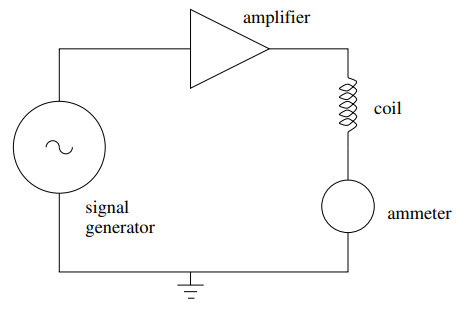
\includegraphics[width=.65\textwidth]{PrimaryCircuit.png}
           \caption{The primary circuit}
           \label{fig:PrimaryCircuitDiagram}
        \end{center}
    \end{figure}
    Additionally, we had our secondary coil connected to an oscilloscope in order to monitor 
    the induced emf $\epsilon$. This search coil was placed on a contraption that allowed us 
    to hold it at set distances from the primary coil, along the primary coil's axis. 

    \section{Experiment}
    \subsection{Field on the Axis of a Circular Coil}\label{sec:FieldAxis}
    In this section we looked specifically at the relationship between magnetic field 
    $\vec{B}(\vec{r},t)$ and induced $\epsilon$. First we look at Faraday's law, which says 
    \begin{equation}
        \epsilon=-N_1\frac{d}{dt}\int\vec{B}\cdot d\vec{A}
        \label{eqn:Faradays Law}
    \end{equation}
    In our case, we are aligning things in a way to have the magnetic field dependent only on 
    the distance $z$ from the primary coil. We also say that the magnetic field is directed 
    along the $z$-axis, approximately, allowing us to consider amplitudes only. So we have 
    \begin{align*}
        B(z,t)&\approx B(z)\cos(\omega t)\\
        \implies \epsilon&\approx -N_a A \frac{d}{dt}(B(z)\cos(\omega t))\\
        &=N_a AB(z)\omega\sin(\omega t)\\
        \implies B(z)&\approx \frac{\epsilon}{N_a A \omega}
    \end{align*}
    where $N_a$ is the number of winds in the search coil (175), $A$ is the cross-sectional 
    area of the search coil, $\omega$ is the angular frequency that the primary coil is being 
    driven at ($2\pi f$), and we have taken $\sin(\omega t)$ to be 1 as we are only interested 
    in amplitudes. We now have a kind of ``calibration factor", so when we measure the emf 
    induced in the search coil, we can immediately know the approximate value of the magnetic 
    field that induced it, i.e. the magnetic field produced by the primary coil. \newline
    We have a way of determining the magnetic field from the induced voltage, but we also want 
    to know how well that method agrees with what we would expect from the primary coil. The 
    magnitude of the magnetic field on the axis of a circular coil of radius $a$ is
    \begin{equation}
        B(z,t)=\frac{\mu_0 N I(t)}{2}\frac{a^2}{(a^2+z^2)^\frac{3}{2}}
        \label{eqn:MagFieldOnAxis}
    \end{equation}
    where $\mu_0=\num{4\pi e-7}$ is the permeability of free space, $N$ is the number of winds
    on the coil (120), and $I(t)=I_0\cos(\omega t)$. Again we can take the $\cos$ term to 
    be 1 as we're looking at amplitudes, which leaves us with 
    \begin{equation*}
        B(z)=\frac{\mu_0 N I_0}{2}\frac{a^2}{(a^2+z^2)^\frac{3}{2}}
    \end{equation*}
    Finally we collected some data: \newline
    We ran the signal generator at 
    $\SI{1000}{\hertz}=\SI{2000\pi}{\radian\second^{-1}}$ and $2V_{pp}$, with the amplifier 
    setting the current to $I_{rms}=\SI{0.353\pm0.02020}{\ampere}=\SI{0.495\pm0.029}{\ampere}$. 
    This uncertainty comes from reading the current off of our ammeter, which displayed 
    $\SI{0.35}{\ampere}$ rms, so we use a digital pdf with uncertainty $\frac{a}{2\sqrt3}$ 
    and $a=0.01$ as well as the 2\% uncertainty rating on the ammeter 
    to find $u(I_{rms})=\sqrt{0.02^2+\frac{0.01}{2\sqrt 3}}=0.02020$, so $u(I_0)=0.02020\sqrt{2}=0.029$. \newline
    The cross-sectional area of the search coil is $A=(\num{6.5e-3})^2\pi=\SI{1.3273\pm0.0204e-4}{\metre^2}$. 
    This uncertainty comes from the uncertainty on the measurement of the diameter of the 
    search coil, using the formula $u(x^n)=|n|x^{n-1}u(x)$. \newline
    The uncertainty on any experimentally determined $B$ comes from the equation 
    \begin{equation*}
        u(B)=u(\frac{\epsilon}{N_a A\omega})=\frac{\epsilon}{N_a A\omega}\sqrt{\left( \frac{u(\epsilon)}{\epsilon}\right)^2+\left( \frac{u(A)}{A}\right)^2+\left( \frac{u(\omega)}{\omega}\right)^2}
    \end{equation*}
    where $u(\omega)$ is 2\% of the scale used on the display of the signal generator, which 
    was $1 kHz$, so $u(\omega)=0.02\cdot2000\pi=40\pi$, and $u(\epsilon)$ is determined from 
    the 2\% uncertainty of the display of the oscilloscope combined with the digital measurement 
    uncertainty
    \begin{align*}
        u(\epsilon)&=\sqrt{0.02^2+\left(\frac{\num{1e-5}}{2\sqrt3}\right)}\\
        &=0.01
    \end{align*}
    The data and the theoretical model are in \autoref{fig:FieldAxisData}.
    \begin{figure}[h]
        \begin{center}
           \scalebox{.7}{\subimport{Data}{FieldAxisData.pgf}}
           \caption{Magnetic field determined using the calibration factor and $\epsilon$ 
           induced in a search coil due to a large primary coil, along with the theoretical 
           prediction made using \autoref{eqn:MagFieldOnAxis}}
           \label{fig:FieldAxisData}
        \end{center}
    \end{figure}
    
    \subsection{Frequency Dependence of Induced Voltage}\label{sec:EmfPropToFreq}
    This section focuses on the effect of varying the frequency of alternating current on the 
    system we're investigating. We suspect that the relationship is linear.
    For simplicity's sake we moved the coil to position $z=0$ and varied the frequency from 
    100 Hz to 2 kHz. We did not operate below 100 Hz as that would lead to the inductive 
    reactance $X_R=L\omega$ to decrease, effectively causing the coil to become a short 
    circuit. The current would spike and the coil would heat up rapidly.
    The current was kept at $I_{rms}=\SI{0.57\pm0.0202}{\ampere}$ so $I_0=\SI{0.806\pm0.029}{\ampere}$ 
    using the same methods as before. This is done to ensure that the magnetic field remains at 
    the same magnitude throughout the experiment. The current needs to be adjusted as we change 
    frequency to keep it the same as $I=\frac{V}{Z}=\frac{V}{\sqrt{R^2+L^2\omega^2}}$, so the 
    current changes with respect to frequency. \newline
    Now onto the experiment: Altering the current at each frequency and finding the induced 
    $\epsilon$ at each $\omega$, we found the plot in \autoref{fig:EmfPropToFreq}. 
    \begin{figure}[H]
        \begin{center}
           \scalebox{.7}{\subimport{Data}{EmfPropToFreq.pgf}}
           \caption{The emf induced in the axial coil due to a changing frequency of alternating 
           current through the primary coil, kept at the same current to preserve the magnitude 
           of the magnetic field.}
           \label{fig:EmfPropToFreq}
        \end{center}
    \end{figure}
    The data is clearly linear. This confirms our earlier suspicion, but now let us check if 
    our gradient calculated from the line of best fit agrees with what we would expect. Our 
    linear least squares fit gave us a value of $m=\num{3.8188\pm0.0104e-05}$. To verify this 
    we will use two methods. We notice that \autoref{eqn:Faradays Law} gives us a relation 
    between induced $\epsilon$ and $\omega$:
    \begin{equation}
        \epsilon=N_aA\omega B(z)
    \end{equation}
    Since we are keeping $B$ constant, we should have a gradient of $m=N_aAB$. $N_a$ and $A$ 
    are the number of winds in the axial coil and the cross-sectional area of the axial coil 
    respectively and are constants. $B$ is also a constant but we have two ways of determining 
    it. Firstly we can find it from the induced $\epsilon$, using our calibration factor from 
    the previous section on each $\epsilon$ and averaging it to find a $B$. Secondly we can 
    use \autoref{eqn:MagFieldOnAxis} where $z=0$, so 
    \begin{equation}
        B=\frac{\mu_0NI_0}{2a}
        \label{eqn:MagFieldAt0}
    \end{equation}
    Using the first method we found $B_1=\SI{1.640\pm0.056e-3}{\tesla}$, so \newline
    $m_1=\num{3.81\pm0.14e-05}$. The uncertainty on $B_1$ is found with 
    \begin{align*}
        u(B_1)&=\frac{1}{n}u(\sum_i B_i) =\frac{1}{n}\sqrt{\sum_i u(B_i)^2}\\
        u(B_i)&=B_i\sqrt{\left( \frac{u(\epsilon)}{\epsilon}\right)^2+\left( \frac{u(A)}{A}\right)^2+\left( \frac{u(\omega)}{\omega}\right)^2}
    \end{align*}
    Using the second method we found $B_2=\SI{1.788\pm0.028e-3}{\tesla}$, so \newline
    $m_2=\num{4.15\pm0.64e-5}$. The uncertainty on $B_2$ is found with
    \begin{equation*}
        u(B_2)=B_2*\sqrt{\left( \frac{u(I_0)}{I_0}\right)^2+\left( \frac{u(a)}{a}\right)^2}
    \end{equation*}
    where $u(I_0)$ is as given above and $u(a)=\frac{u(d_{primary})}{2}=\SI{0.05e-2}{\metre}$.
    \begin{table}[H]
        \centering
        \begin{tabular}{c c}
            Experimental: & $m_E = \num{3.8188\pm0.0104e-05}$\\
            Expected: & $m_1 = \num{3.81\pm0.14e-05}$\\
            & $m_2 = \num{4.15\pm0.64e-5}$
        \end{tabular}
        \caption{The experimental and two theoretical determinations of the gradient of 
        induced voltage $\epsilon$ with respect to $\omega$, the angular frequency of the AC voltage}
        \label{tbl:ExpectedGradients}
    \end{table}
    
    \subsection{Resistance and Inductance of the Primary Coil}\label{sec:ResistanceInductance}
    This section focuses in on the primary coil as we aimed to determine the resistance and 
    inductance of the primary coil. We used the same set-up as the previous section.
    To do this we look at the equation
    \begin{align*}
        V&=IZ\\
        &=I\sqrt{R^2+L^2\omega^2}
    \end{align*}
    and see that, since we have kept the current constant, we have $V$ as a function of $\omega$, 
    with $R$ and $L$ as parameters that we can optimise using \texttt{scipy.optimize.curve\_fit}. 
    Using the data from before, but this time with the voltage across the primary coil, we have 
    \autoref{fig:ResistanceInductance}.
    \begin{figure}[H]
        \begin{center}
           \scalebox{.7}{\subimport{Data}{ResistanceInductance.pgf}}
           \caption{The amplitude of the voltage across the primary coil as a function 
           of the angular frequency $\omega$, with the \texttt{curve\_fit} approximation 
           of a line of best fit using the Jackknife method.}
           \label{fig:ResistanceInductance}
        \end{center}
    \end{figure}
    The error on the experimental data is a result of the limitations of the oscilloscope display 
    and the uncertainty associated with digital measurement, given by 
    \begin{equation*}
        u(V_{\text{primary}})=\frac{\sqrt{\left(\frac{0.01}{2\sqrt 3}\right)^2+2^2}}{2}
    \end{equation*}
    Note the division by 2 that's necessary as the data was recorded as a $V_{pp}$, so we divide 
    it by 2 to find the amplitude, and thus divide the uncertainty by 2. \newline
    \texttt{curve\_fit} gives us the following values for $R$ and $L$, with the uncertainties 
    coming from the Jackknife method of error approximation.
    \begin{table}
        \centering
        \begin{tabular}{c c}
            Resistance: & $\SI{3.3326\pm0.0085}{\ohm}$\\
            Inductance: & $\SI{1.50820\pm0.00037e-3}{\henry}$
        \end{tabular}
        \caption{Resistance and inductance of the primary coil determined using 
        \texttt{curve\_fit} on the emf across the primary coil when varying the frequency 
        of AC voltage input, keeping current the same.}
        \label{tbl:ResistanceInductance}
    \end{table}

    \section{Discussion and Recommendations}
    \subsection{Field on the Axis of a Circular Coil}
    Examining \autoref{fig:FieldAxisData} we see that for the most part our experimental data 
    agrees comfortably with the theoretical prediction within experimental uncertainty. Most 
    importantly, they have a very similar shape and both have a maximum at $z=0$, which 
    makes sense considering magnetic field is inversely proportional to distance, in the most 
    basic form. \newline
    To improve the results of this experiment, we would recommend using a larger axial coil 
    as it would then cover more of the magnetic field, as well as not making approximations 
    when modifying Faraday's Law. This should lead to more accurate predictions of the fringe 
    effects of magnetic field, which can be prominent.

    \subsection{Frequency Dependence of Induced Voltage}
    The linear least squares fit in \autoref{fig:EmfPropToFreq} fits well to the data, the 
    uncertainty on the experimentally determined gradient being $\sim 0.2\%$ of the value. 
    Regarding the expected values in \autoref{tbl:ExpectedGradients}, $m_1$ agrees with 
    the $m_E$ to an almost suspicious degree, but this makes sense since we 
    used the calibration factor in the calculation of both the experimental and expected 
    values. What's really interesting is that $m_2$ agrees with $m_E$ within experimental 
    uncertainty. This confirms that the methods we used to determine these values experimentally 
    were valid. \newline
    The same improvements as in the previous section would improve these results. It's clear 
    that the theoretical prediction of $m$ is greater than that of $m$ found using the 
    approximation in Faraday's Law, meaning that our approximation underestimates the 
    magnitude of the magnetic field. 

    \subsection{Resistance and Inductance of the Primary Coil}
    The results in \autoref{tbl:ResistanceInductance} seem quite reasonable for a coil of wire. 
    We don't expect a large resistance value, and inductance is usually on the scale of 
    $\num{1e-3}$. Our confidence in these values is confirmed by the small uncertainties. \newline
    There is not much that can be done to improve this section of the experiment except for an 
    improvement in the accuracy of the tools used to measure the values, which should give us 
    lower uncertainty values.

    \section{Conclusion}
    To conclude, this experiment produced values which agreed with their theoretical 
    counterparts, when there were predictions for the values at least, and values which 
    make sense considering the physical attributes of the apparatus used. We accurately 
    determined the relationship between the magnetic field produced by a coil of wire 
    driven by and AC voltage and the voltage induced in a second coil oriented in the same 
    direction as the primary coil. We confirmed that the relationship between induced voltage 
    and frequency of the AC supply current in that circuit is linear, and found values for 
    the resistance and inductance of the primary coil. 

    \newpage
    \section{Appendix}
    \setcounter{figure}{0} \renewcommand{\thefigure}{A.\arabic{figure}}
    \lstinputlisting[caption=Code for \autoref{sec:FieldAxis},label=app:FieldAxis,style=appendix]{FieldAxis.py}
    \lstinputlisting[caption=Code for \autoref{sec:EmfPropToFreq},label=app:EmfPropToFreq,style=appendix]{EmfPropToFreq.py}
    \lstinputlisting[caption=Code for \autoref{sec:ResistanceInductance},label=app:ResistanceInductance,style=appendix]{ResistanceInductance.py}
    

\end{document}